\documentclass[journal]{IEEEtran}

\usepackage{cite}
\usepackage{graphicx}
\usepackage{amsmath,amssymb}
\usepackage{booktabs}
\usepackage{multirow}
\usepackage[hyphens]{url}
% All experiments, controls and tables are part of the main article.

% Fall back to the bundled Computer Modern typewriter face when the optional
% Courier metrics are unavailable in a minimal TeX installation.
\renewcommand{\ttdefault}{cmtt}

% IEEEtran uses 8 pt (\footnotesize) text for journal tables. Keep all result
% tables on the same typography and spacing settings without geometric scaling.
\newcommand{\resulttablesetup}{%
  \footnotesize
  \setlength{\tabcolsep}{2pt}%
  \renewcommand{\arraystretch}{1.15}%
}

% Compact float placement without changing IEEE body typography or margins.
\setcounter{topnumber}{3}
\setcounter{dbltopnumber}{3}
\setcounter{totalnumber}{5}
\renewcommand{\topfraction}{0.9}
\renewcommand{\dbltopfraction}{0.9}
\renewcommand{\textfraction}{0.08}
\renewcommand{\floatpagefraction}{0.75}
\renewcommand{\dblfloatpagefraction}{0.75}
\setlength{\floatsep}{10pt plus 2pt minus 2pt}
\setlength{\dblfloatsep}{10pt plus 2pt minus 2pt}
\setlength{\textfloatsep}{12pt plus 2pt minus 2pt}
\setlength{\dbltextfloatsep}{12pt plus 2pt minus 2pt}
\makeatletter
\setlength{\@fptop}{0pt}
\setlength{\@fpsep}{12pt}
\setlength{\@fpbot}{0pt plus 1fil}
\setlength{\@dblfptop}{0pt}
\setlength{\@dblfpsep}{12pt}
\setlength{\@dblfpbot}{0pt plus 1fil}
\makeatother

\hyphenation{text-to-motion auto-regressive MotionGPT}

\title{COMPASS: Relation-Conditioned Prompt Robustness for Text-to-Motion Generation}

\author{Anonymous Authors}

\markboth{IEEE Transactions on Multimedia,~Vol.~XX, No.~XX, 2026}%
{Anonymous Authors: COMPASS}

\begin{document}

\maketitle

\begin{abstract}
Text-to-motion generators should tolerate meaning-preserving prompt rewrites
while responding to intentional semantic edits. We introduce COMPASS, a
relation-conditioned fine-tuning framework that uses early motion-token
likelihoods to compute text-token attribution. It combines attribution-weighted
alignment for preserving pairs, edit-local objectives for altering pairs, and a
frozen teacher, while retaining the motion tokenizer and generator
architecture. A local analysis relates the
forward alignment loss to projected Jacobian energy and derives sufficient
conditions for risk reduction and token-distribution stability. We evaluate
preserving rewrites on HumanML3D, Motion-X, and KIT-ML with classifier-free
guidance fixed to 1.3. After independent native text-encoder adaptation,
COMPASS variants exceed their parents in mean top-three retrieval (R@3) across
lexical, syntactic, and narrative rewrites: the margins are 11.89 and 1.97
percentage points on HumanML3D, and 0.85 and 1.69 points on Motion-X, for the
T2M-GPT and MotionGPT families. These estimates use one generation seed and
20 shared random candidate partitions. Separate tests before text adaptation
show dataset-dependent FID trade-offs; the quality and retrieval columns
therefore describe distinct configurations. A frozen-text diagnostic finds
30.3\% lower mean hidden-state cosine displacement, but also shows that the
detached attribution losses do not directly update the generator. The results
support checkpoint-specific paraphrase robustness while leaving causal
attribution and motion-level semantic-edit compliance unresolved.
\end{abstract}

\begin{IEEEkeywords}
Text-to-motion generation, prompt robustness, meaning-preserving rewrites,
motion-conditioned attribution, cross-dataset prompt robustness.
\end{IEEEkeywords}

\section{Introduction}
Text-to-motion generation converts natural-language descriptions into human
motion, enabling animation and interactive motion
creation~\cite{zhang2023generating,tevet2022humanmotiondiffusionmodel}.
In an interactive setting, a user may revise the wording of a prompt without
changing the intended action, or edit a specific action attribute. Reliable
control requires distinguishing these two cases. For example, ``walk forward
slowly'' and ``move ahead at a slow pace'' should express similar motions;
replacing ``forward'' with ``backward'' should instead change direction while
retaining the action and speed. We call this requirement \emph{selective
prompt robustness}: invariance to preserving rewrites and sensitivity to
intentional semantic edits.

Standard caption--motion likelihood training provides no explicit supervision
for this relation between prompts. T2M-GPT represents motion with a
vector-quantized variational autoencoder (VQ-VAE) and predicts discrete motion
tokens from CLIP text features~\cite{zhang2023generating,radford2021learning}.
Each caption is supervised by its target motion, but the objective does not
specify which changes in language should preserve that target. SATO addresses
instability under synonyms and small textual perturbations by regularizing
text attention and motion prediction~\cite{chen2024sato}. Extending such
invariance to intentional edits, however, can conflict with the requested
change. The relation between prompts must therefore determine the form of
regularization.

A second challenge is choosing the signal to regularize. Text similarity and
attention alone do not identify which words support a particular generated
motion. We use the likelihood of the target motion's early autoregressive
tokens to compute Grad~$\times$~Input attribution. This yields a
motion-conditioned, model-dependent measure of textual evidence. COMPASS uses
that evidence to weight auxiliary text representations, aligns them for
preserving pairs, and defines attribution-change and locality objectives for
edited and unedited positions in altering pairs. A frozen teacher limits
prediction drift. The framework retains the pretrained motion tokenizer and
generator architecture.

The evaluation distinguishes the proposed objective from the effects that
can be established for its implementations. The T2M-GPT-family source models
use frozen CLIP features and detached attribution gradients. Separate native
text-encoder adaptation updates CLIP for T2M-GPT and T5 for MotionGPT before
retrieval evaluation. All generation tests use classifier-free guidance
(CFG) at 1.3; the FID columns use source encoders before this additional stage,
whereas retrieval and the other columns use adapted encoders. These column
groups describe different generated actions. Across three rewrite levels,
the adapted COMPASS variants have higher retrieval point estimates than their
parents on HumanML3D and Motion-X. Source-encoder FID results instead show
dataset- and backbone-dependent trade-offs. KIT-ML, component comparisons,
and frozen HumanML3D-to-KIT text transfer test the scope of these observations.

To interpret prompt stability, we derive local connections between cosine
alignment, projected Jacobian energy, and token-distribution variation.
The analysis states the extra conditions needed to transfer auxiliary
consistency to the generator. We then examine those conditions with
hidden-state, Jacobian, and gradient-connectivity diagnostics. The detached
configuration has lower measured hidden-state sensitivity, but its attribution
losses have no direct gradient path to the generator. This finding separates
a useful conditional interpretation from a verified causal training mechanism.

Our contributions are threefold:
\begin{itemize}
    \item We formulate selective prompt robustness through preserving and
    altering relations, and introduce COMPASS, which combines motion-conditioned
    attribution with relation-specific objectives and teacher regularization.
    \item We provide caption-locked evaluations across three datasets,
    separating source-encoder quality from adapted-encoder retrieval, and
    report both improvements and configuration-dependent regressions.
    \item We derive conditional local stability bounds and use internal
    diagnostics to test their applicability, identifying the gradient-path
    limitation of the reported detached-attribution configuration.
\end{itemize}

\section{Related Work}
\subsection{Text-to-Motion Generation and Control}
Text-to-motion models differ in how they represent and generate motion.
MotionDiffuse and the Human Motion Diffusion Model use continuous
 diffusion~\cite{zhang2022motiondiffusetextdrivenhumanmotion,tevet2022humanmotiondiffusionmodel}.
T2M-GPT quantizes motion and predicts tokens autoregressively, while
MotionGPT treats motion tokens as a language within a pretrained
language-model framework~\cite{zhang2023generating,jiang2023motiongpt}.
MoMask and MMM use iterative masked-token completion rather than
left-to-right prediction~\cite{guo2024momask,pinyoanuntapong2024mmmgenerativemaskedmotion}.
These approaches motivate evaluating prompt robustness across more than one
text-conditioning architecture.

Motion control and editing provide a related but distinct setting.
OmniControl imposes joint-level spatial constraints~\cite{xie2024omnicontrol};
SALAD uses skeleton-aware latent diffusion for generation and
editing~\cite{hong2025salad}. MotionFix learns from source motions, edit
instructions, and edited targets, and SimMotionEdit studies text-based editing
with motion-similarity prediction~\cite{athanasiou2024motionfix,li2025simmotionedittextbasedhumanmotion}.
COMPASS instead regularizes paired prompts for a pretrained generator. It does
not require an edited target motion for each altering pair, but this weaker
supervision also limits what can be concluded about motion-level edit
compliance.

\subsection{Prompt Robustness and Relation Supervision}
SATO identifies sensitivity to synonymous wording and small text
perturbations in text-to-motion generation~\cite{chen2024sato}. Its invariance
objective motivates our preserving branch. Intentional semantic edits require
a different response: stabilizing a changed action or direction can suppress
the requested control signal. Contrast sets and counterfactually augmented
data similarly distinguish changes that test a decision boundary from
variations that should leave a prediction
unchanged~\cite{gardner2020evaluatingmodelslocaldecision,kaushik2019learning}.
Our relation labels make this distinction explicit in prompt-pair training.
The main generation tests evaluate preserving rewrites; altering pairs inform
the objective and internal diagnostics rather than a benchmark with edited
motion ground truth.

\subsection{Attribution and Representation Regularization}
Gradient-based attribution describes the local dependence of a selected
score on the input, with interpretation that depends on the model and
attribution procedure~\cite{sundararajan2017axiomatic,adebayo2018sanity}.
COMPASS applies Grad~$\times$~Input to target-motion likelihood rather than a
text-only score. Its preserving objective applies stop-gradient Siamese
alignment to the resulting motion-conditioned
representations~\cite{chen2021exploring}.
Teacher matching constrains prediction drift, following the broader principle
of learning without forgetting~\cite{li2017learning}.
The contribution is the relation-conditioned use of these components, not a
new attribution estimator. Their forward objectives and effective gradient
paths are distinguished in our method and diagnostics.

\section{Method}
\subsection{Problem Formulation}
Let $x$ denote a text prompt and let $y=(y_1,\ldots,y_T)$ denote the discrete
motion-token sequence obtained from a pretrained VQ-VAE tokenizer. T2M-GPT
models the conditional distribution
\begin{equation}
    p_{\theta}(y\mid x)=\prod_{t=1}^{T}p_{\theta}(y_t\mid y_{<t}, x),
\end{equation}
where the text condition is produced by a CLIP text encoder and the motion
tokens are predicted autoregressively. COMPASS fine-tunes the autoregressive
generator rather than replacing the VQ-VAE or the decoding pipeline.

A training example is $(x,x',y,r,m)$: $x'$ is a paired prompt,
$r\in\{\mathrm{preserve},\mathrm{alter}\}$ is its relation to $x$, and $m$
marks edited text positions. Preserving pairs retain the original action
semantics. Altering pairs change one action, direction, or body-part slot.
For either relation, $y$ is the original motion used to compute attribution;
for an altering pair it is not an edited-motion target. The broader motivation
includes speed, count, and temporal order, but these factors are not separately
evaluated here. Relation labels specify whether the prompt-pair objective
should encourage agreement or edit-local sensitivity.

\subsection{Framework Overview}
Figure~\ref{fig:framework} summarizes the T2M-GPT-family implementation.
The trainable modules are the autoregressive Transformer, including its output
head, an auxiliary projection $\phi$, and a predictor $q$. The source models
studied here freeze CLIP and the VQ-VAE; subsequent text-only adaptation is a
separate stage described in Section~\ref{sec:independent_adaptation}.
A teacher Transformer is initialized from the same pretrained checkpoint as
the student and remains frozen.

Each mini-batch contributes a generation loss on the original prompts. When
attribution objectives are active, both prompts are encoded and scored against
the original motion tokens. The relation label selects preserving alignment
or altering difference/locality losses. A frozen teacher regularizes the
resulting training objective. The auxiliary heads
are used only during training, so the motion vocabulary, tokenizer, and
inference architecture remain unchanged.

% TODO(figure): regenerate sato++.png. The current raster still draws the
% variance and covariance panels in the preserve branch, which were removed
% from the objective. The caption below flags this until the image is redrawn.
\begin{figure*}[t]
\centering
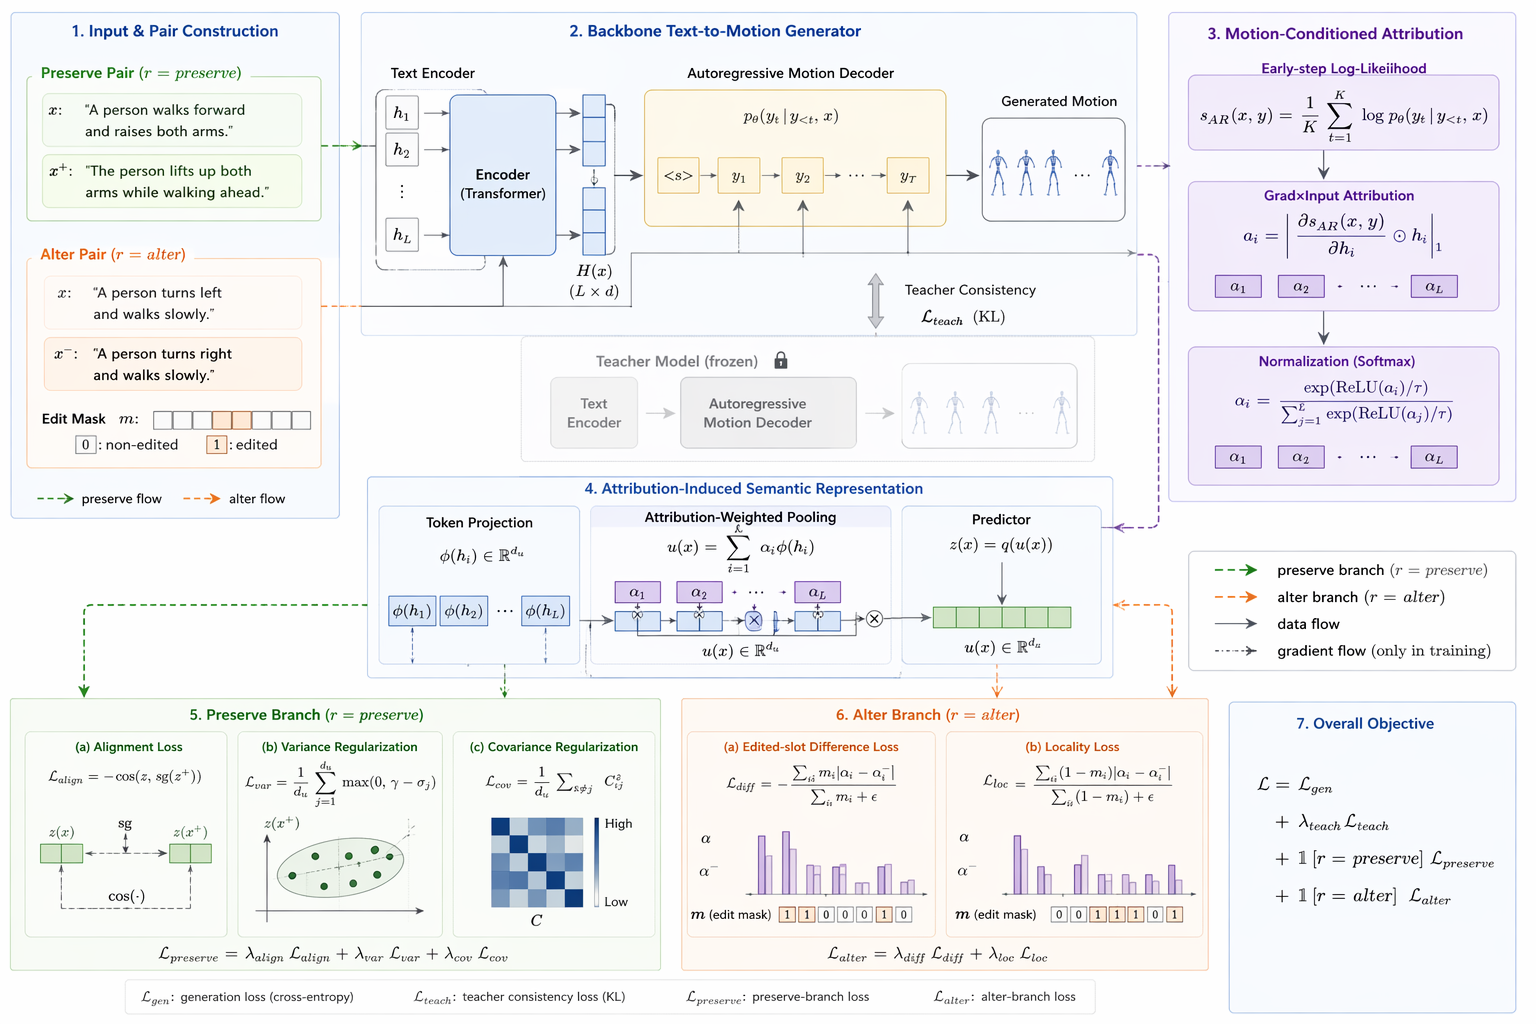
\includegraphics[width=\linewidth]{sato++.png}
\caption{COMPASS training framework. Early target-motion likelihoods provide
Grad~$\times$~Input weights for auxiliary text representations. Preserving
pairs use attribution-weighted alignment; altering pairs
use edited-position differences and unedited-position locality. A frozen
teacher constrains prediction drift. The schematic's KL teacher label applies
to the Motion-X MotionGPT preserve-only variant; T2M-GPT-family sources use
L1 logit matching. The variance and covariance panels drawn in the preserve
branch are not part of the objective reported here.
Attribution-gradient connectivity is configuration dependent.}
\label{fig:framework}
\end{figure*}

\subsection{Motion-Conditioned Token Attribution}
We derive token weights from the generator's likelihood of a particular target
motion. For prompt $x$ and motion tokens $y$, the attribution score averages
the first $K$ autoregressive predictions:
\begin{equation}
    s_{\mathrm{AR}}(x,y)=
    \frac{1}{K}\sum_{t=1}^{K}\log p_{\theta}(y_t\mid y_{<t},x),
\end{equation}
where $K$ is restricted to valid target-token positions. Let $h_i$ denote the
input CLIP token embedding at position $i$, distinct from the generator hidden
state $h_\theta$ used later. Grad~$\times$~Input assigns
\begin{equation}
    a_i(x,y)=
    \left\lVert
    \frac{\partial s_{\mathrm{AR}}(x,y)}{\partial h_i}\odot h_i
    \right\rVert_1 .
\end{equation}
The raw attribution values are converted into a probability distribution over
text positions:
\begin{equation}
    \alpha_i(x,y)=
    \frac{\exp(\mathrm{ReLU}(a_i)/\tau)}
    {\sum_j \exp(\mathrm{ReLU}(a_j)/\tau)} ,
\end{equation}
where $\tau$ is a temperature. Because the score is a target-motion likelihood,
$\alpha$ weights textual evidence relevant to that motion under the current
model. It is a local attribution measure, not a ground-truth importance label.
The distinction between differentiating through these weights and treating
them as constants is specified below.

\subsection{Attribution-Weighted Semantic Representation}
COMPASS pools token features with the attribution distribution:
\begin{equation}
    u(x,y)=\sum_i \alpha_i(x,y)\,\phi(H_i(x)),
\end{equation}
where $H_i(x)$ is the contextual CLIP feature and $\phi$ projects it into the
auxiliary representation space. A predictor produces
\begin{equation}
    z(x,y)=q(u(x,y)).
\end{equation}
The predictor is used for preserving alignment, following the stop-gradient
Siamese formulation~\cite{chen2021exploring}.

\subsection{Preserving Branch}
For $r=\mathrm{preserve}$, the paired prompts should describe the same target
motion even if they use different surface forms. COMPASS aligns their
motion-conditioned representations with a stop-gradient cosine objective:
\begin{equation}
    \mathcal{L}_{\mathrm{align}}
    =-\cos\bigl(z(x,y),\mathrm{sg}(z(x',y))\bigr),
\end{equation}
where $\mathrm{sg}(\cdot)$ denotes stop-gradient. The preserving objective
weights this alignment term:
\begin{equation}
    \mathcal{L}_{\mathrm{pres}}
    =
    \lambda_{\mathrm{align}}\mathcal{L}_{\mathrm{align}} .
\end{equation}
Cosine alignment alone admits a constant-representation solution. The
stop-gradient asymmetry between the two branches is the only structural
constraint against it here, and it does not guarantee that collapse is
avoided.

\subsection{Altering Branch}
For $r=\mathrm{alter}$, the edited slot should remain influential. Let
$m_i\in\{0,1\}$ indicate whether token position $i$ belongs to the edited slot.
COMPASS encourages attribution to change on edited positions:
\begin{equation}
    \mathcal{L}_{\mathrm{diff}}
    =
    -
    \frac{\sum_i m_i|\alpha_i(x,y)-\alpha_i(x',y)|}
    {\sum_i m_i+\epsilon}.
\end{equation}
The negative sign means that minimizing this term increases attribution
difference on the edited slot. At the same time, COMPASS penalizes attribution
drift outside the edited slot:
\begin{equation}
    \mathcal{L}_{\mathrm{loc}}
    =
    \frac{\sum_i (1-m_i)|\alpha_i(x,y)-\alpha_i(x',y)|}
    {\sum_i (1-m_i)+\epsilon}.
\end{equation}
The altering objective is
\begin{equation}
    \mathcal{L}_{\mathrm{alter}}
    =
    \lambda_{\mathrm{diff}}\mathcal{L}_{\mathrm{diff}}
    +
    \lambda_{\mathrm{loc}}\mathcal{L}_{\mathrm{loc}} .
\end{equation}
The negative sign rewards differences at edited positions, while the locality
term penalizes differences elsewhere. These losses specify a desired
attribution response to semantic edits; motion-level compliance requires
separate evaluation.

\subsection{Teacher-Preserved Fine-Tuning Objective}
The base generation loss is the T2M-GPT cross-entropy over target motion tokens,
\begin{equation}
    \mathcal{L}_{\mathrm{gen}}
    =
    -\sum_{t=1}^{T}\log p_{\theta}(y_t\mid y_{<t},x).
\end{equation}
To protect generation quality during robustness fine-tuning, the student is
regularized toward a frozen teacher. In the main T2M-GPT-family result reported
here, this teacher term is an L1 distance between student and teacher logits over
valid motion-token positions:
\begin{equation}
    \mathcal{L}_{\mathrm{teach}}
    =
    \frac{1}{T}\sum_t
    \left\lVert \ell_{\theta,t}-\ell_{\mathrm{teacher},t}\right\rVert_1 .
\end{equation}
The overall COMPASS loss is
\begin{equation}
    \mathcal{L}
    =
    \mathcal{L}_{\mathrm{gen}}
    +\lambda_{\mathrm{teach}}\mathcal{L}_{\mathrm{teach}}
    +\mathbf{1}_{r=\mathrm{preserve}}\mathcal{L}_{\mathrm{pres}}
    +\mathbf{1}_{r=\mathrm{alter}}\mathcal{L}_{\mathrm{alter}} .
\end{equation}
This equation describes the T2M-GPT-family objective used for the main COMPASS
checkpoints.  The MotionGPT plug-in reported in
Table~\ref{tab:motionx_methods} is a distinct preserve-only variant: it adds
paired-caption generation loss on $x'$, uses a KL teacher term, retains the
preserving alignment term, and sets the altering loss
weights to zero.  We therefore do not use that row as evidence for the full
preserve-plus-alter objective.

\subsection{Implementation and Gradient Paths}
The T2M-GPT-family source configurations use $K=16$, frozen CLIP and VQ-VAE
weights, L1 teacher matching, and
\texttt{attribution\_create\_graph=false}. Edit masks are mapped from annotated
words to CLIP positions. Detaching the score gradient removes the
second-order path through attribution. With CLIP also frozen, the attribution
objectives update auxiliary heads but have no direct gradient path to the
generator in the audited implementation. Generation and teacher losses supply
the generator updates (Section~\ref{sec:detail_attribution_details}).
The Motion-X MotionGPT preserve-only variant enables the attribution graph
and uses its own native text and motion components. We retain these
implementation distinctions when interpreting both the theory and results.

\subsection{Conditional Theory of Preserving-Prompt Robustness}
\label{sec:robustness_theory}
We separate the geometry of a consistency loss, the conditions under which
its update can improve a generator, and the consequences of hidden-state
stability for output probabilities. These are local, conditional statements,
not an assumption that the detached implementation satisfies their premises.

\paragraph{Local coordinates and hidden-state geometry.}
Fix target tokens, teacher-forced prefixes, text positions, and attention
masks. Let $e$ concatenate visible continuous text embeddings and $h_\theta(e)$
concatenate final generator states over fixed valid motion positions. Its
Euclidean norm corresponds to the Frobenius norm used in our diagnostics.
Let $\delta$ be a perturbation in these embedding coordinates and let
$\mathcal U_{\rm pres}$ be the local subspace spanned by embedded preserving
prompt differences. Its span need not consist entirely of valid semantic
edits. We assume twice continuously differentiable maps with bounded
derivatives on the analyzed neighborhood and nonzero basepoint norms for
both hidden and auxiliary representations. These assumptions exclude
nondifferentiable points of the attribution map; finite token replacements
need not satisfy the small-perturbation approximation. Define
\begin{equation}
\begin{aligned}
 r_\theta(e,\delta)&=\frac{\|h_\theta(e+\delta)-h_\theta(e)\|_2}
 {\|h_\theta(e)\|_2},\\
 \widetilde J_\theta&=\frac{\partial h_\theta(e)/\partial e}{\|h_\theta(e)\|_2}.
\end{aligned}
\label{eq:theory_relative_jacobian}
\end{equation}
The denominator is held fixed: $\widetilde J$ is not the Jacobian of
$h/\|h\|$. Taylor expansion gives
\begin{equation}
 r_\theta^2=\delta^\top\widetilde J_\theta^\top\widetilde J_\theta\delta
 +O(\|\delta\|_2^3).
\label{eq:theory_local_response}
\end{equation}
For class $c$ at basepoint $e$, let $S_c=\mathbb E[\delta\delta^\top\mid e,c]$.
The identity $v^\top Av=\operatorname{tr}(Avv^\top)$ yields
\begin{equation}
 \mathbb E[r_\theta^2\mid e,c]
 =\operatorname{tr}(\widetilde J_\theta S_c\widetilde J_\theta^\top)
 +O(\mathbb E[\|\delta\|_2^3\mid e,c]).
\label{eq:theory_trace}
\end{equation}
For centered perturbations $S_c$ is the covariance; otherwise it also
includes the mean outer product. Different token classes therefore probe
different directions of a common local map.

\paragraph{Proposition 1: the forward value of cosine alignment.}
Set $\bar z=z/\|z\|_2$ and $J_{\bar z}=\partial\bar z/\partial e$ with
$y$ fixed. The preserving loss satisfies
\begin{equation}
\begin{aligned}
 1+\mathcal L_{\rm align}
 &=\tfrac12\|\bar z(e+\delta,y)-\bar z(e,y)\|_2^2\\
 &=\tfrac12\delta^\top J_{\bar z}^\top J_{\bar z}\delta
 +O(\|\delta\|_2^3).
\end{aligned}
\label{eq:theory_alignment}
\end{equation}
\emph{Proof.} Unit vectors obey $\|a-b\|_2^2=2-2a^\top b$.
Substitute $\bar z(e+\delta)=\bar z(e)+J_{\bar z}\delta+O(\|\delta\|^2)$.
Its expectation is one half of
$\operatorname{tr}(J_{\bar z}S_{\rm pres}J_{\bar z}^\top)$ to leading order.
The loss value thus measures data-dependent projected Jacobian energy.
Stop-gradient preserves this value but changes its parameter derivative:
this is not an equivalence between the actual detached update and gradient
descent on a fully differentiated Jacobian penalty~\cite{chen2021exploring}.

For the differentiable forward pooling map, the chain rule gives
\begin{equation}
 J_u=\sum_i\alpha_i J_{\phi\circ H_i}
 +\sum_i\phi(H_i)(\nabla_e\alpha_i)^\top.
\label{eq:theory_pooling_jacobian}
\end{equation}
Motion-conditioned weights allocate sensitivity according to the current
model's target-likelihood evidence, not ground-truth semantic importance.
Retaining the attribution-gradient graph can introduce mixed second
likelihood derivatives; detaching it removes this path while leaving any
remaining trainable feature/head paths. Consistent normalized attribution
maps alone do not bound the magnitude of the underlying input gradient.

Small $J_{\bar z}$ does not automatically imply small generator Jacobian
$J_h$. A sufficient additional bridge is
\begin{equation}
 \|J_h v\|_2\le\kappa\|J_{\bar z}v\|_2,
 \qquad v\in\mathcal U_{\rm pres}.
\label{eq:theory_bridge}
\end{equation}
For instance, this holds if the relevant local map factors as $h=f(\bar z)$
with $\|J_f\|_2\le\kappa$; merely sharing parameters is insufficient.
Then expected squared hidden drift is bounded by
$2\kappa^2\mathbb E[1+\mathcal L_{\rm align}]$ plus a third-order remainder.
We do not assume this factorization for COMPASS's auxiliary pooling head.

\paragraph{Proposition 2: sufficient cross-class contraction.}
Let subscripts $0,+$ denote the parent and COMPASS at the same input and
prefixes. Suppose that on $\mathcal U_{\rm pres}$,
\begin{equation}
 \widetilde J_+^\top\widetilde J_+
 \preceq\gamma^2\widetilde J_0^\top\widetilde J_0,
 \qquad 0<\gamma<1.
\label{eq:theory_contraction}
\end{equation}
Then $r_+\le\gamma r_0+O(\|\delta\|_2^2)$ for every sufficiently small
direction in the subspace. Expected squared responses satisfy the analogous
bound with factor $\gamma^2$, up to a third-order remainder, for each class
supported there. \emph{Proof.} The positive-semidefinite ordering bounds
$\|\widetilde J_+\delta\|_2$ by $\gamma\|\widetilde J_0\delta\|_2$;
Taylor expansion and the triangle inequality give the response bound, and
\eqref{eq:theory_trace} gives its expectation. Approximate proportionality
$\widetilde J_+\approx\gamma Q\widetilde J_0$, $Q^\top Q=I$, is a stronger
possible explanation for similar relative reductions across classes.
Neither similar class means nor smaller individual spectral norms establish
the directional ordering in~\eqref{eq:theory_contraction}.

\paragraph{Proposition 3: conditional risk reduction by an attribution update.}
Let $\theta_g$ contain only generator parameters, with auxiliary parameters
fixed during the comparison. Let $R(\theta_g)$ be a differentiable average
risk under a fixed preserving-perturbation distribution, such as perturbed
cross-entropy or $\mathbb E[r_\theta^2]$, rather than worst-case adversarial
risk. Let $a_g$ be the gradient delivered by the implemented attribution
objective to $\theta_g$, including stop-gradient choices, and
$b_g=\nabla_{\theta_g}R$. If $R$ is $\beta$-smooth along the update segment,
then for $\lambda>0$ and step size $\eta\ge0$,
\begin{equation}
\begin{aligned}
 R(\theta_g-\eta\lambda a_g)-R(\theta_g)
 \le{}&-\eta\lambda\langle b_g,a_g\rangle\\
 &+\tfrac12\beta\eta^2\lambda^2\|a_g\|_2^2.
\end{aligned}
\label{eq:theory_descent}
\end{equation}
\emph{Proof.} Apply the smoothness descent lemma with increment
$-\eta\lambda a_g$. Positive $\langle b_g,a_g\rangle$ ensures strict
reduction for sufficiently small steps. For $\beta>0$, it suffices that
$0<\eta<2\langle b_g,a_g\rangle/(\beta\lambda\|a_g\|_2^2)$.
This is an attribution-only Euclidean update, not a guarantee for a joint
Adam update, whose effective direction must be considered separately.
If $a_g=0$, the generator update is zero and its gradient cosine is undefined.
Our frozen-CLIP detached-attribution audit finds this disconnected case
(Section~\ref{sec:detail_attribution_details}); the strict-descent premise is
therefore unavailable for that configuration.

\paragraph{Proposition 4: conditional output-distribution bounds.}
At a shared autoregressive prefix $v$, write $h_t=h_{\theta,t}(e;v)$ and
$h_t'=h_{\theta,t}(e+\delta;v)$. Suppose
$\|\ell_t-\ell_t'\|_2\le M_t\|h_t-h_t'\|_2$ in the neighborhood;
for a linear head one may take $M_t=\|W_t\|_2$. Define the unit-temperature
probabilities $p_t=\operatorname{softmax}(\ell_t)$ and
$p_t'=\operatorname{softmax}(\ell_t')$. With $\operatorname{CE}$ denoting
cross-entropy and $D_{\rm KL}$ Kullback--Leibler divergence,
\begin{equation}
\begin{aligned}
 D_{\rm KL}(p_t\|p_t')&\le\tfrac14 M_t^2\|h_t-h_t'\|_2^2,\\
 |\operatorname{CE}(\ell_t',y_t)-\operatorname{CE}(\ell_t,y_t)|
 &\le\sqrt{2}M_t\|h_t-h_t'\|_2.
\end{aligned}
\label{eq:theory_output_bounds}
\end{equation}
\emph{Proof.} For $A(\ell)=\log\sum_j\exp(\ell_j)$,
$\nabla^2A=\operatorname{diag}(p)-pp^\top$ has spectral norm at most $1/2$.
Thus $D_{\rm KL}(p\|p')=D_A(\ell',\ell)\le\|\ell'-\ell\|_2^2/4$,
where $D_A$ is the Bregman divergence generated by $A$.
Also $\|\nabla_\ell\operatorname{CE}\|_2=\|p-e_{y_t}\|_2\le\sqrt2$,
where $e_{y_t}$ is the one-hot target vector.
For fixed horizon $T$ (or absorbing EOS padding), the KL chain rule yields
\begin{equation}
 D_{\rm KL}(P_e\|P_{e+\delta})
 \le\tfrac14\sum_{t=1}^T M_t^2
 \mathbb E_{v\sim P_e}[\|h_t-h_t'\|_2^2],
\label{eq:theory_sequence_kl}
\end{equation}
provided the bounds hold at every prefix in the expectation. Here $P_e$ is
the sequence law and both conditionals use the same sampled prefix $v$.
Measurements at selected target prefixes alone do not verify this premise.
Guidance requires bounds on its actual combined logits; truncation changes
the probability law. These statements do not certify individual sampled
trajectories or imply monotone FID, diversity, or retrieval gains. Comparing
models also requires accounting for their different head norms $M_t$.

\paragraph{Roles and limits of the remaining regularizers.}
By the triangle inequality, the student's prompt-pair logit difference is at
most the teacher's difference plus the two student--teacher residuals.
Teacher matching limits drift but does not guarantee improvement over the
teacher.
Altering losses prefer edit-local evidence changes, not a proven lower bound
on motion-level edit response. The theoretical scope is the evaluated
preserving-perturbation family, not global invariance or certified semantic
control.


\section{Experiments}
\label{sec:experiments}
The experiments address three questions: how COMPASS source models respond to
preserving rewrites, how independently adapted text encoders affect retrieval,
and whether internal diagnostics support the proposed stability mechanism.
We report generation quality and retrieval for explicitly distinguished
configurations, then examine component choices, text-domain transfer, and
hidden-state behavior.

\subsection{Experimental Setup}
\label{sec:independent_adaptation}
\label{sec:detail_protocol_details}

\paragraph{Datasets and prompt pairs.}
We use HumanML3D~\cite{guo2022generating}, Motion-X~\cite{lin2023motionx}, and
KIT-ML~\cite{plappert2016kit}, with native 263-, 322-, and 251-dimensional
motion representations. Preserving rewrites are grouped into lexical changes
(P1), syntactic changes (P2), and narrative-style changes (P3). The mixed
HumanML3D and Motion-X tests contain 4,380 and 7,679 caption-locked motions:
each motion has a fixed original caption, rewrite, and crop. Before testing,
seed 123 assigns one rewrite per motion, giving P1/P2/P3 counts of
1,460/1,460/1,460 and 2,560/2,560/2,559. Each mixture is evaluated as a
single dataset, rather than by averaging level-specific metrics.
Native KIT retains 734 full-motion pairs from 830 entries under its native
length rules. The separate 734-pair transfer set uses the archived P2/P3
pairing; it is not interchangeable with the native mixture. Pair order,
normalization, and source checkpoints are fixed before generation.

\paragraph{Source and adapted configurations.}
A \emph{source configuration} uses each model's text encoder before the
additional text-only adaptation stage. An \emph{adapted configuration} updates
that model's native text encoder: CLIP for the T2M-GPT family and T5 for the
MotionGPT family. Encoders are independent across models. The FID variants in
the mixed-result tables use source configurations; every other column,
including retrieval, Matching, diversity, and transfer pair/token measures,
uses adapted configurations. Both share prompts, generation settings, and the
frozen motion evaluator, but generate separate actions. The column-wise
reporting was revised after inspection of the adapted results. Both complete
result sets are retained. The T2M-GPT+COMPASS source checkpoint was
subsequently reselected from a sweep of thirteen training endpoints scored on
this mixture, so that row is a test-selected endpoint and its margins are
optimistic; all other rows retain their pre-declared endpoints.

\paragraph{Text-only adaptation.}
Each native text encoder receives 3,000 updates with equal-weight
original/rewrite action-token prediction on training-only preserving pairs.
The generation backbone, VQ-VAE, auxiliary heads, and CLIP visual branch remain
frozen; for T5, the shared embeddings, decoder, and output layer also remain
frozen. This stage does not reapply COMPASS losses. HumanML3D, KIT, and component
variants use learning rate $10^{-6}$, 100 warmup steps, and a fixed endpoint.
Motion-X retains the previously validation-selected configurations, including
T5 learning rates $3\times10^{-5}$ for MotionGPT and $10^{-6}$ for
MotionGPT+COMPASS. Only matching training annotations and valid native motion
tokens are admitted; held-out motions and mirrored sources are excluded.
The Motion-X MotionGPT+COMPASS source is the preserve-only variant described in
the method. Component sources retain their differing original training budgets.

\paragraph{Generation.}
Every test uses generation seed 123 and CFG $s=1.3$, applied to conditional
and unconditional logits as $\ell_u+s(\ell_c-\ell_u)$. Original and rewritten
conditions reset the same deterministic per-batch random seed. T2M-GPT uses
zero CLIP features for its unconditional branch. For MotionGPT, an
inference-time branch retains \texttt{Generate motion:} but removes the
description and uses the same decoder prefix. At CFG=1, the wrapper reproduces
the original MotionGPT generation path. This extension does not imply that
these T5 checkpoints were trained with unconditional-caption dropout, and the
two architectures have different unconditional inputs. Native motion
tokenizers, length rules, and normalization are preserved, including KIT's
251-dimensional representation at 12.5 frames per second.

\paragraph{Shared evaluators.}
All models within a dataset use the same frozen text--motion matching
evaluator. Its text encoder is adapted to training clean/preserving pairs;
its movement and motion encoders retain standard weights. Word lookup first
tries the original form and falls back to lowercase only on failure.
HumanML3D and KIT retain alphabetic-token filtering; Motion-X retains its
non-alphabetic-inclusive processing. Evaluator adaptation and lookup correction
are distinct from adapting the generator's CLIP or T5 encoder.

For KIT evaluator selection, 288 eligible official validation motions provide
864 P1/P2/P3 rewrites generated and filtered with \texttt{gemini-3.1-flash-lite}.
These texts are used only for validation. Evaluator text training uses 20
rounds of 200 updates at learning rate $10^{-4}$; a batch contains eight
unique motions, each with clean/P1/P2/P3 text, and rolled negatives from
different motions. The predeclared acceptance criteria allow at most a
one-percentage-point clean R@1 drop, require a macro rewrite R@1 gain of at
least 0.5 points, and require P3 nonregression. Round 20 is selected: clean
R@1 increases from 42.53\% to 43.77\%, and macro rewrite R@1 from 26.00\%
to 39.18\%. These are real-motion validation scores, not generator gains.
Motion-side parameter hashes and save/reload consistency are verified.

% Float placement policy: each wide table is declared roughly one subsection
% ahead of the text that discusses it. IEEE two-column table* floats can only
% reach the top of a later page, so declaring them at the point of discussion
% pushed them one to two pages downstream.
\begin{table*}[t]
\centering
\caption{HumanML3D on 4,380 fixed prompt pairs, CFG=1.3. FID variants use source encoders; other columns use adapted encoders and separate generations. Retrieval (\%) averages 20 candidate partitions of one generation seed. Bold marks the within-family best; diversity is closest to the real reference (9.137).}
\label{tab:humanml_methods}
\resulttablesetup
\begin{tabular*}{\textwidth}{@{\extracolsep{\fill}}l*{8}{c}@{}}
\toprule
Method & \multicolumn{3}{c}{Source encoder} & \multicolumn{5}{c}{Adapted encoder} \\
\cmidrule(lr){2-4}\cmidrule(lr){5-9}
 & FID $\downarrow$ & FID$_P$ $\downarrow$ & FID$_D$ $\downarrow$ & Matching$_P$ $\downarrow$ & R@1$_P$ $\uparrow$ & R@2$_P$ $\uparrow$ & R@3$_P$ $\uparrow$ & Div.$_O$ \\
\midrule
T2M-GPT & \textbf{0.080} & 0.233 & 0.190 & 4.169 & 36.36 & 52.15 & 61.76 & 8.421 \\
T2M-GPT+COMPASS & 0.147 & \textbf{0.170} & \textbf{0.132} & \textbf{3.462} & \textbf{45.11} & \textbf{63.23} & \textbf{72.89} & \textbf{9.340} \\
\midrule
MotionGPT & 0.741 & 0.670 & \textbf{0.111} & 4.449 & 34.29 & 50.41 & 60.07 & \textbf{9.410} \\
MotionGPT+COMPASS & \textbf{0.516} & \textbf{0.371} & 0.167 & \textbf{4.263} & \textbf{36.09} & \textbf{52.76} & \textbf{62.29} & 9.527 \\
\bottomrule
\end{tabular*}

\end{table*}

\paragraph{Metrics and reporting.}
Fr\'echet inception distance (FID) is computed in the evaluator's motion
embedding space. FID compares original-caption generations with the real
motions, FID$_P$ compares rewrite generations with those real motions, and
FID$_D$ compares the two generated distributions. Each uses the entire fixed
mixture. Matching$_P$ is the mean Euclidean distance from each rewritten text
to the motion generated from that text. R@1/2/3$_P$ reports whether that motion
is among the top one, two, or three retrieved candidates. Queries and their
corresponding generated motions are jointly shuffled into 20 shared random
partitions, with at most 32 candidates per group and the final partial group
retained. Reported R-Precision percentages are averages across partitions of
one generation, not estimates over 20 generation seeds.

Diversity$_O$ uses original-caption generations from the adapted configuration
and a fixed seed for 300 sampled index pairs. Lower FID and Matching are
preferred; diversity is assessed by proximity to the real-motion reference.
Bold entries mark the best point estimates under each caption's comparison
rule, not statistically significant differences. FID values are compared only
within a dataset's embedding space. No generation-seed variance or paired
significance claim is reported.

\subsection{HumanML3D: Quality and Alignment}
\begin{table*}[t]
\centering
\caption{Motion-X on 7,679 fixed prompt pairs with a shared evaluator, CFG=1.3. FID variants use source encoders; other columns use adapted encoders. Bold marks the within-family best as in Table~\ref{tab:humanml_methods}; real diversity is 14.322.}
\label{tab:motionx_methods}
\resulttablesetup
\begin{tabular*}{\textwidth}{@{\extracolsep{\fill}}l*{8}{c}@{}}
\toprule
Method & \multicolumn{3}{c}{Source encoder} & \multicolumn{5}{c}{Adapted encoder} \\
\cmidrule(lr){2-4}\cmidrule(lr){5-9}
 & FID $\downarrow$ & FID$_P$ $\downarrow$ & FID$_D$ $\downarrow$ & Matching$_P$ $\downarrow$ & R@1$_P$ $\uparrow$ & R@2$_P$ $\uparrow$ & R@3$_P$ $\uparrow$ & Div.$_O$ \\
\midrule
T2M-GPT & 0.203 & 1.279 & 0.813 & 5.182 & 40.40 & 57.88 & 67.79 & 14.232 \\
T2M-GPT+COMPASS & \textbf{0.166} & \textbf{0.804} & \textbf{0.586} & \textbf{5.110} & \textbf{41.00} & \textbf{58.79} & \textbf{68.75} & \textbf{14.398} \\
\midrule
MotionGPT & \textbf{2.618} & 3.750 & 0.596 & 7.553 & 21.60 & 34.80 & 44.23 & \textbf{13.134} \\
MotionGPT+COMPASS & 2.775 & \textbf{3.338} & \textbf{0.109} & \textbf{7.324} & \textbf{22.68} & \textbf{36.06} & \textbf{45.73} & 13.053 \\
\bottomrule
\end{tabular*}

\end{table*}
Table~\ref{tab:humanml_methods} shows improved rewrite quality with different
costs across backbones. With source encoders, T2M-GPT+COMPASS lowers FID$_P$
from 0.233 to 0.170 and FID$_D$ from 0.190 to 0.132, while original-caption
FID increases from 0.080 to 0.147. MotionGPT+COMPASS lowers FID from 0.741
to 0.516 and FID$_P$ from 0.670 to 0.371, but increases FID$_D$ from 0.111
to 0.167. Thus closer rewrite generations to real motion do not require a
smaller gap between original- and rewrite-generated distributions.
In the adapted configurations, R@3$_P$ increases from 61.76\% to 72.89\%
for the T2M-GPT family and from 60.07\% to 62.29\% for the MotionGPT family.

\subsection{Motion-X: Dependence on Text Adaptation}
\begin{table*}[t]
\centering
\caption{HumanML3D retrieval after independent text adaptation, CFG=1.3. Each level has 4,380 prompt--motion pairs, one generation seed, and 20 shared random candidate partitions of at most 32, with the tail retained. The rewritten text is used for both generation and retrieval. Bold marks the within-family best point estimate. Values are percentages.}
\label{tab:humanml_independent_cfg}
\resulttablesetup
% Source: ablation/humanml_independent_cfg13_20260907/humanml_summary.csv
% SHA256: 8047349e39dec33d8feff6ee551e219f219cf86722e3dbc1684028f4250bda58
% Percent; one generation seed (123), averaged over 20 random candidate partitions.
\begin{tabular*}{\textwidth}{@{\extracolsep{\fill}}ll*{9}{c}@{}}
\toprule
Method & Encoder & \multicolumn{3}{c}{P1} & \multicolumn{3}{c}{P2} & \multicolumn{3}{c}{P3} \\
\cmidrule(lr){3-5}\cmidrule(lr){6-8}\cmidrule(lr){9-11}
& & R@1 & R@2 & R@3 & R@1 & R@2 & R@3 & R@1 & R@2 & R@3 \\
\midrule
T2M-GPT & CLIP & 35.54 & 50.95 & 60.47 & 42.78 & 59.64 & 69.01 & 29.29 & 43.83 & 53.49 \\
T2M-GPT + COMPASS & CLIP & \textbf{45.14} & \textbf{63.18} & \textbf{72.93} & \textbf{50.47} & \textbf{69.87} & \textbf{79.36} & \textbf{39.04} & \textbf{56.43} & \textbf{66.36} \\
\midrule
MotionGPT & T5 & 36.95 & 53.56 & 63.30 & 37.48 & 53.84 & 63.43 & 29.60 & 44.07 & 53.43 \\
MotionGPT + COMPASS & T5 & \textbf{37.48} & \textbf{54.06} & \textbf{63.98} & \textbf{39.69} & \textbf{56.92} & \textbf{66.63} & \textbf{30.75} & \textbf{45.97} & \textbf{55.48} \\
\bottomrule
\end{tabular*}

\end{table*}
\begin{table*}[t]
\centering
\caption{Motion-X retrieval on 7,679 pairs per level, using the protocol in Table~\ref{tab:humanml_independent_cfg} and the frozen Motion-X paraphrase-aware evaluator with lowercase fallback. Bold marks the within-family best. Values are point estimates in percent, not generation-seed means and deviations.}
\label{tab:motionx_independent_cfg}
\resulttablesetup
% Source: ablation/motionx_independent_cfg13_20260907/motionx_summary.csv
% SHA256: 0b4327846b6836176df4489ac8cf78eefcab4e453d477bf6022139a2d931d0a7
% Percent; one generation seed (123), averaged over 20 random candidate partitions.
\begin{tabular*}{\textwidth}{@{\extracolsep{\fill}}ll*{9}{c}@{}}
\toprule
Method & Encoder & \multicolumn{3}{c}{P1} & \multicolumn{3}{c}{P2} & \multicolumn{3}{c}{P3} \\
\cmidrule(lr){3-5}\cmidrule(lr){6-8}\cmidrule(lr){9-11}
& & R@1 & R@2 & R@3 & R@1 & R@2 & R@3 & R@1 & R@2 & R@3 \\
\midrule
T2M-GPT & CLIP & 42.55 & 60.69 & 70.73 & 48.04 & 67.18 & 76.85 & 30.85 & 46.75 & 56.99 \\
T2M-GPT + COMPASS & CLIP & \textbf{42.60} & \textbf{60.74} & \textbf{70.78} & \textbf{48.61} & \textbf{67.92} & \textbf{77.69} & \textbf{31.92} & \textbf{48.34} & \textbf{58.66} \\
\midrule
MotionGPT & T5 & 23.11 & 36.57 & 46.26 & 24.76 & 39.23 & 49.27 & 17.05 & 28.46 & 37.13 \\
MotionGPT + COMPASS & T5 & \textbf{23.98} & \textbf{37.95} & \textbf{48.08} & \textbf{25.80} & \textbf{40.77} & \textbf{51.04} & \textbf{17.94} & \textbf{29.71} & \textbf{38.62} \\
\bottomrule
\end{tabular*}

\end{table*}
With source encoders, T2M-GPT+COMPASS improves all three FID measures in
Table~\ref{tab:motionx_methods}: FID/FID$_P$/FID$_D$ are 0.166/0.804/0.586,
compared with 0.203/1.279/0.813 for its parent. MotionGPT+COMPASS lowers
FID$_P$ from 3.750 to 3.338 and FID$_D$ from 0.596 to 0.109, while increasing
original-caption FID from 2.618 to 2.775. The adapted configurations improve
R@3$_P$ from 67.79\% to 68.75\% and from 44.23\% to 45.73\% for the
two families, respectively.

A controlled pre/post-CLIP comparison explains why configuration matters.
Holding prompts, real embeddings, evaluator, CFG, and seed fixed, the
T2M-GPT-family FID ranking reverses after independent text adaptation.
Both generation backbones remain unchanged during that stage. Recomputed
summaries match the saved embeddings, and an independent float64 FID
calculation differs by less than $10^{-6}$. The checked numerical and
reference-embedding explanations therefore do not account for the reversal.
The source FID advantage cannot be combined with adapted retrieval gains as
evidence of one jointly superior system; the complete adapted FID results
remain in the experiment archive.

\subsection{Retrieval by Rewrite Level}
\begin{table*}[t]
\centering
\caption{Native KIT-ML on 734 prompt pairs, CFG=1.3, using the shared KIT evaluator selected on official validation data. FID variants use source encoders; other columns use adapted encoders and separate generations. Bold marks the column best; diversity is closest to 11.148. Retrieval is in percent.}
\label{tab:cross_dataset}
\resulttablesetup
\begin{tabular*}{\textwidth}{@{\extracolsep{\fill}}lrrrrrrrr@{}}
\toprule
Method & FID $\downarrow$ & FID$_P$ $\downarrow$ & FID$_D$ $\downarrow$ & Matching$_P$ $\downarrow$ & R@1$_P$ $\uparrow$ & R@2$_P$ $\uparrow$ & R@3$_P$ $\uparrow$ & Div.$_O$ \\
\midrule
T2M-GPT & 0.454 & 1.330 & 1.352 & 3.543 & 34.64 & 54.05 & 65.44 & \textbf{11.308} \\
MotionGPT & 1.265 & 1.446 & \textbf{0.260} & 6.343 & 22.92 & 35.93 & 44.55 & 11.395 \\
T2M-GPT+COMPASS & \textbf{0.396} & \textbf{1.194} & 1.270 & \textbf{3.323} & \textbf{36.31} & \textbf{56.48} & \textbf{68.54} & 11.358 \\
\bottomrule
\end{tabular*}

\end{table*}
The per-level tests evaluate each rewrite type on all 4,380 HumanML3D or
7,679 Motion-X motions (Tables~\ref{tab:humanml_independent_cfg}
and~\ref{tab:motionx_independent_cfg}). They use the same adapted checkpoints,
CFG, and evaluator as the mixed-table retrieval columns. Each level has its
own prompt and candidate population, so a mixed-test score is not the macro
average of the level-specific scores.

COMPASS variants have higher retrieval point estimates than their respective
parents at every rank and rewrite level. On HumanML3D, mean P1/P2/P3 R@3
increases from 60.99\% to 72.88\% for the T2M-GPT family and from 60.06\%
to 62.03\% for the MotionGPT family. The corresponding Motion-X changes are
68.19\% to 69.04\% and 44.22\% to 45.91\%. The gains span all three
rewrite types, with larger margins for the HumanML3D T2M-GPT family. They
characterize these adapted checkpoints and do not isolate individual losses
or variability across training and generation seeds.

\subsection{Native KIT-ML Evaluation}
\begin{table*}[t]
\centering
\caption{Contextual HumanML3D component comparison on 4,380 prompt pairs. FID variants use source encoders; other columns use adapted encoders. Parent/main rows reuse Table~\ref{tab:humanml_methods}. Source budgets and endpoints differ, precluding a matched causal ablation. Bold marks the column best; diversity is closest to 9.137.}
\label{tab:main_results}
\resulttablesetup
\begin{tabular*}{\textwidth}{@{\extracolsep{\fill}}lrrrrrrrr@{}}
\toprule
Method & FID $\downarrow$ & FID$_P$ $\downarrow$ & FID$_D$ $\downarrow$ & Matching$_P$ $\downarrow$ & R@1$_P$ $\uparrow$ & R@2$_P$ $\uparrow$ & R@3$_P$ $\uparrow$ & Div.$_O$ \\
\midrule
T2M-GPT & \textbf{0.080} & 0.233 & 0.190 & 4.169 & 36.36 & 52.15 & 61.76 & 8.421 \\
Synonym augmentation & 0.224 & 0.263 & \textbf{0.031} & 3.471 & 44.54 & 63.26 & 73.11 & 9.400 \\
T2M-GPT+COMPASS & 0.147 & \textbf{0.170} & 0.132 & 3.462 & 45.11 & 63.23 & 72.89 & 9.340 \\
w/o preserve & 0.240 & 0.244 & 0.102 & 3.440 & 45.24 & 63.76 & \textbf{73.47} & 9.311 \\
w/o attribution & 0.248 & 0.268 & 0.137 & \textbf{3.423} & \textbf{45.47} & \textbf{63.77} & 73.43 & \textbf{9.231} \\
w/o teacher & 0.208 & 0.219 & 0.108 & 3.520 & 44.62 & 62.57 & 72.16 & 9.310 \\
w/o alter & 0.219 & 0.235 & 0.111 & 3.493 & 44.42 & 62.71 & 72.62 & 9.494 \\
\bottomrule
\end{tabular*}

\end{table*}
The native KIT test supports a source-encoder quality advantage for the
T2M-GPT-family COMPASS model (Table~\ref{tab:cross_dataset}): FID/FID$_P$/FID$_D$
decrease from 0.454/1.330/1.352 to 0.396/1.194/1.270. MotionGPT obtains
FID$_P$ 1.446. With adapted encoders, the T2M-GPT-family Matching$_P$ decreases
from 3.543 to 3.323 and R@3$_P$ increases from 65.44\% to 68.54\%; MotionGPT
attains 44.55\% R@3$_P$. These generator comparisons share the same evaluator
and are separate from its validation improvement.

\subsection{Component and Augmentation Comparisons}
\label{sec:detail_component_removal}
\begin{table*}[t]
\centering
\caption{HumanML3D-to-KIT text transfer on 734 P2/P3 pairs, without KIT generator adaptation. FID$_D$ uses HumanML3D source encoders; other columns use HumanML3D-adapted encoders and separate generations. The HumanML3D evaluator is frozen. Bold marks the better value in each column under the direction given in its header. Retrieval and first-token agreement are percentages.}
\label{tab:human_to_kit}
\resulttablesetup
\begin{tabular*}{\textwidth}{@{\extracolsep{\fill}}lrrrrrrr@{}}
\toprule
Method & FID$_D$ $\downarrow$ & Matching$_P$ $\downarrow$ & R@1$_P$ $\uparrow$ & R@2$_P$ $\uparrow$ & R@3$_P$ $\uparrow$ & Paired $\ell_2$ $\downarrow$ & First token (\%) $\uparrow$ \\
\midrule
T2M-GPT & 0.247 & 3.692 & 34.71 & 51.58 & 61.90 & 3.740 & \textbf{29.70} \\
T2M-GPT+COMPASS & \textbf{0.135} & \textbf{2.968} & \textbf{39.25} & \textbf{58.49} & \textbf{70.31} & \textbf{2.762} & 24.66 \\
\bottomrule
\end{tabular*}
\end{table*}
The component suite exhibits metric-dependent rankings rather than consistent
advantages for the complete objective (Table~\ref{tab:main_results}). With
source encoders, synonym augmentation has lower FID$_D$ than the main COMPASS
row (0.031 versus 0.132), but higher FID$_P$ (0.263 versus 0.170).
With adapted encoders, synonym augmentation, removal of preserving losses,
and removal of attribution give R@3$_P$ of 73.11\%, 73.47\%, and 73.43\%,
compared with 72.89\% for the main model.

These rows also indicate that the parent's original-caption FID advantage is
partly a checkpoint-selection effect rather than an effect of the COMPASS
objective. The released parent is the endpoint selected on best clean FID,
whereas every other row is a continued fine-tune selected under a different
rule. The synonym-augmentation control, which applies no COMPASS loss, reaches
FID 0.224 at its own best-FID checkpoint and 0.181 at its final iteration;
both exceed the 0.147 of the main COMPASS row. Continued training on this
backbone therefore costs original-caption FID on its own, and the COMPASS
objective retains more of it than the augmentation control does.

Each variant retains its locked source endpoint. Additional text adaptation
uses the same action-token prediction objective and does not reactivate
removed losses. Standardizing this stage and evaluation does not equalize
prior generator training budgets. The comparisons therefore characterize
these checkpoints, rather than isolating the causal effect of each loss.

\subsection{HumanML3D-to-KIT Text-Domain Transfer}
\label{sec:detail_zero_shot}
\begin{figure*}[t]
\centering
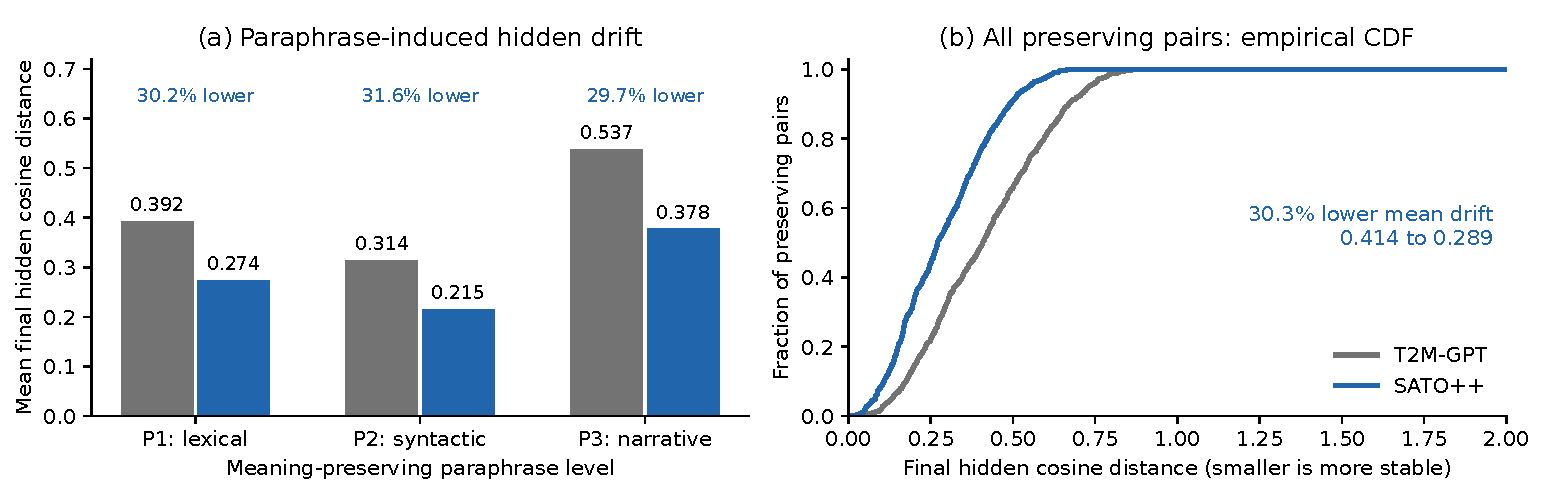
\includegraphics[width=\textwidth]{figures/paraphrase_latent_stability.pdf}
\caption{Lower hidden-state cosine displacement under preserving rewrites for the frozen-CLIP COMPASS checkpoint. The 900-pair diagnostic uses identical target prefixes and reports per-level means and the empirical cumulative distribution; it is separate from adapted-encoder generation evaluation.}
\label{fig:latent_stability}
\end{figure*}
\begin{figure*}[t]
\centering
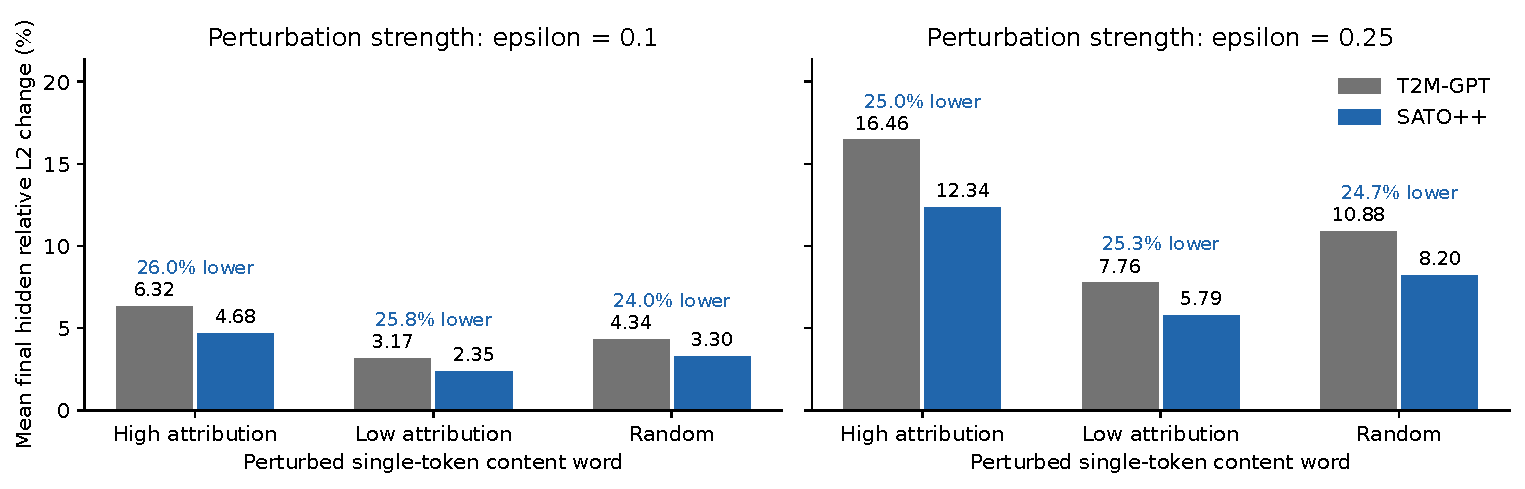
\includegraphics[width=\textwidth]{figures/attribution_guided_local_response.pdf}
\caption{Local input sensitivity on 100 shared groups. Interventions have norms 0.1 and 0.25 times the sentence-median content-word embedding norm. COMPASS has smaller mean relative responses in each condition. High/low ranks are model dependent; random-word identities and directions are shared.}
\label{fig:local_response}
\end{figure*}
The transfer test contains 364 P2 and 370 P3 pairs. HumanML3D-trained models
generate HumanML3D-format motion from KIT descriptions, using the frozen
HumanML3D evaluator throughout. With source encoders, COMPASS lowers FID$_D$
from 0.247 to 0.135 (Table~\ref{tab:human_to_kit}). With adapted encoders,
R@3$_P$ increases from 61.90\% to 70.31\% and paired embedding distance
decreases from 3.740 to 2.762, while first-token agreement decreases from
29.70\% to 24.66\%. Even within the adapted configuration, better embedding
alignment does not imply greater token agreement. Native FID/FID$_P$ are
omitted because no HumanML3D-format KIT real-motion reference is available.
This is text-domain transfer, rather than skeleton retargeting.

\subsection{Hidden-State Stability}
\label{sec:latent_diagnostics}
\begin{figure*}[t]
\centering
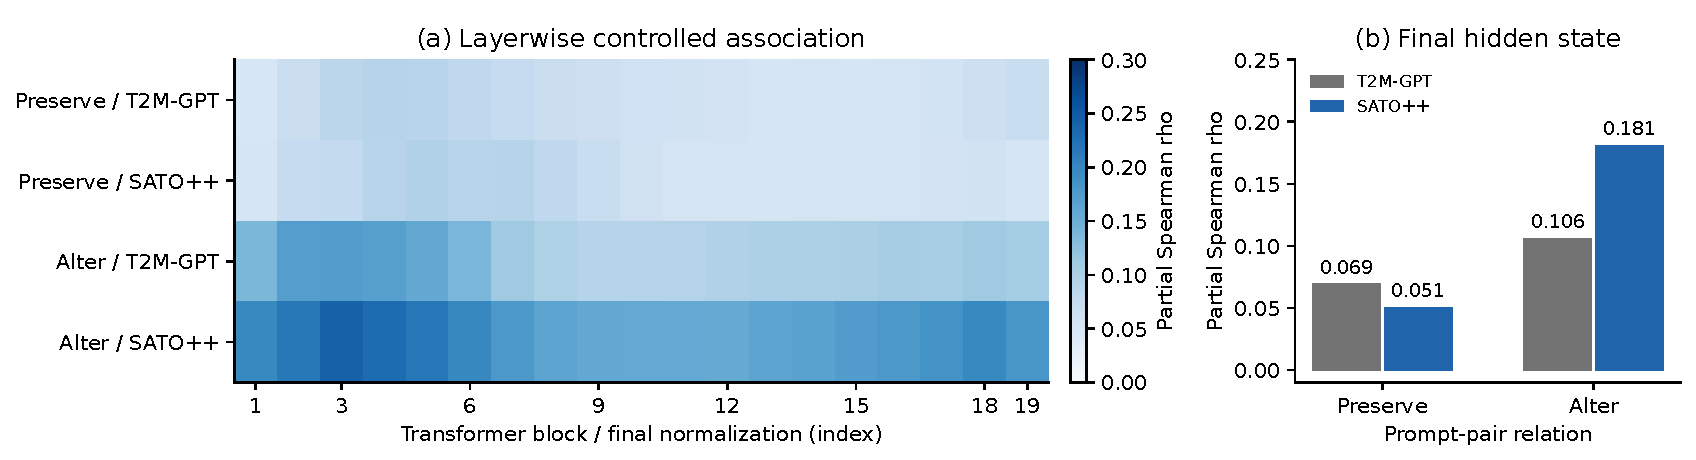
\includegraphics[width=\textwidth]{figures/relation_specific_association.pdf}
\caption{Association between attribution JSD and hidden-state cosine displacement for 900 preserving and 235 rule-edited pairs. (a) Partial rank correlations across 18 Transformer blocks and final normalization. (b) Final-state correlations. The between-model difference for altering pairs is uncertain; both panels use a common scale.}
\label{fig:attribution_association}
\end{figure*}
To examine internal sensitivity, we use the frozen-CLIP parent and a COMPASS
130k checkpoint before additional text adaptation. This mechanism analysis
retains the earlier training endpoint rather than the generation checkpoint
of Table~\ref{tab:humanml_methods}, so it characterizes the objective rather
than that specific row. The fixed HumanML3D subset
contains 300 held-out source-motion groups and 900 preserving pairs, one
P1/P2/P3 pair per group; original and mirrored motions share a group.
Both prompts receive the same teacher-forced target prefix. Mean final-state
cosine displacement over the first 16 valid positions decreases from 0.414
to 0.289 (30.3\%), with per-level reductions of 30.2\%, 31.6\%, and 29.7\%
(Figure~\ref{fig:latent_stability}).
On 100 shared groups, equal-norm interventions on high-attribution,
low-attribution, and random single-token words yield 24.0--26.0\% lower mean
relative hidden-state responses for COMPASS (Figure~\ref{fig:local_response}).
Both models remain more responsive to high- than low-attribution words.
Similar class-level reductions are compatible with shared local sensitivity
reduction in~\eqref{eq:theory_trace}, but do not prove the directional ordering
in~\eqref{eq:theory_contraction}: high/low positions are model dependent, and
continuous embedding interventions are not certified semantic-preserving edits.
The two experiments measure different quantities. Since
$1-\cos(a,b)=\|\bar a-\bar b\|_2^2/2$, a 30\% reduction in mean cosine
distance corresponds to approximately $1-\sqrt{0.70}=16.3\%$ reduction in
root-mean-square normalized chord length, not a 30\% reduction in mean
Euclidean distance. Section~\ref{sec:detail_attribution_details} examines
whether gradient connectivity and direct Jacobian estimates support a common
mechanism behind these observations.
\subsection{Attribution and Jacobian Diagnostics}
\label{sec:detail_attribution_details}
\begin{figure*}[t]
\centering
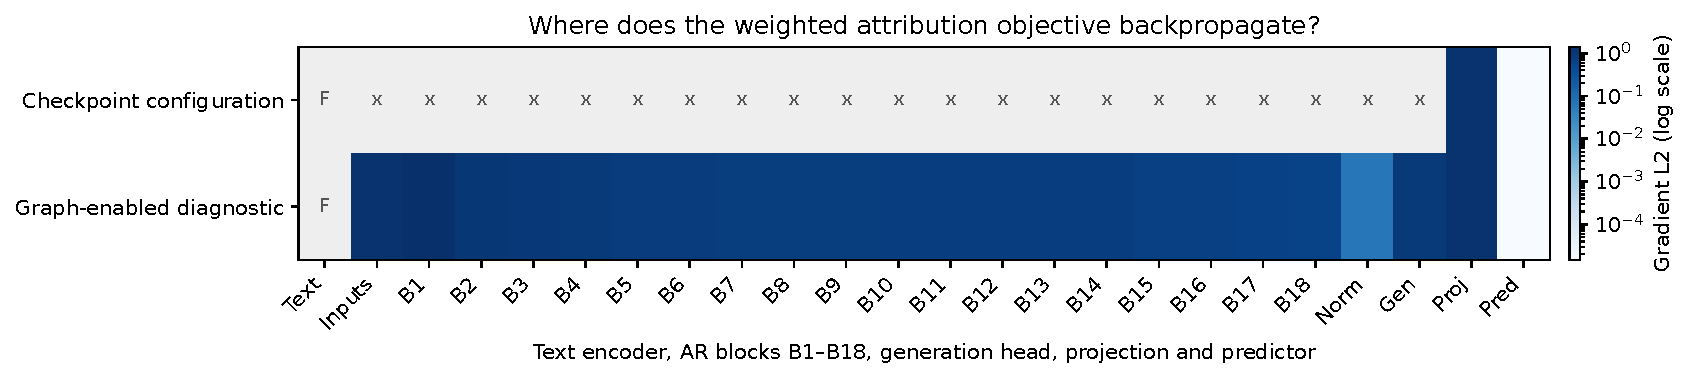
\includegraphics[width=\textwidth]{figures/attribution_gradient_reachability.pdf}
\caption{The detached attribution objective reaches auxiliary heads but not the generator. Colors show gradient $\ell_2$ norms on a logarithmic scale; ``F'' denotes a frozen module and ``x'' a disconnected path. The second row enables the attribution graph only for a same-batch connectivity test, not a newly trained model.}
\label{fig:gradient_reachability}
\end{figure*}
We test the theoretical interpretation at three levels: association between
attribution and hidden-state changes, gradient reachability of the auxiliary
objective, and direct estimates of the text-to-hidden-state Jacobian.

\paragraph{Sampling and representations.}
The 300 source-motion groups in Section~\ref{sec:latent_diagnostics} exclude
training groups and treat original/mirrored motions as one source. Selection
uses seed 123 with a test-specific offset, excluding captions that require
CLIP truncation and motions that require submotion or resampling repairs.
The frozen VQ-VAE encodes deterministic multiple-of-four center crops.
Both text conditions use identical target prefixes. Attribution averages
log-likelihood over at most 16 valid motion tokens per sample, excluding end
and padding tokens. We extract outputs from 18 Transformer blocks and final
normalization.

The 100-group intervention subset requires at least three alphabetic,
non-stopword content words, each occupying one CLIP token. One word is
perturbed at a time, with norm 0.1 or 0.25 times the median eligible-word
embedding norm, three paired Gaussian directions, and both signs.
The relative response divides the Frobenius norm of the hidden-state change
by the unperturbed-state norm. Input strengths, random-word identities, and
directions are shared across models; high/low choices follow each model's
attribution ranking.

\paragraph{Attribution--state association.}
A deterministic single-word rule supplies 235 additional altering pairs:
78 action, 79 body-part, and 78 direction edits. These pairs have no edited
motion ground truth. Attribution comparison excludes special/padding tokens,
normalizes the remaining scores, aligns identical words by occurrence, and
merges unmatched words into a residual bucket. This lexical alignment differs
from the learned pooling head's normalization over all 77 CLIP positions.
We measure Jensen--Shannon divergence (JSD) between the aligned attribution
distributions and its association with hidden-state displacement.

\begin{figure*}[t]
\centering
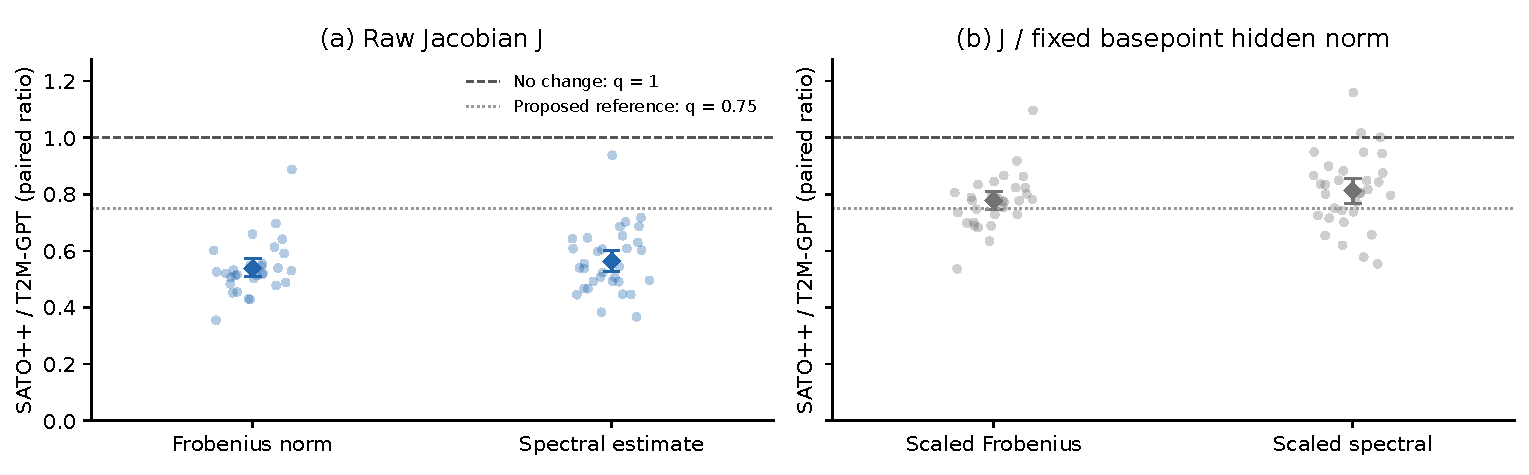
\includegraphics[width=\textwidth]{figures/jacobian_norm_ratios.pdf}
\caption{Lower average local sensitivity for COMPASS on 32 shared groups. (a) Paired ratios of raw Jacobian Frobenius norms and spectral estimates. (b) Ratios after dividing each Jacobian by its model's fixed basepoint hidden norm. Dots denote groups, diamonds means, and bars 95\% source-group bootstrap intervals. The 0.75 line is a reference hypothesis.}
\label{fig:jacobian_norms}
\end{figure*}
Figure~\ref{fig:attribution_association} reports partial Spearman correlations
controlling for frozen CLIP distance, token-count difference, lexical edit
fraction, original token count, valid prefix length, and uniform-attribution
JSD. Final-state correlations for altering pairs are 0.106 for the parent and
0.181 for COMPASS; preserving-pair values are 0.069 and 0.051. For COMPASS,
95\% source-group bootstrap intervals from 1,000 resamples are
$[0.032,0.301]$ and $[-0.021,0.128]$, respectively. The altering-pair
between-model difference is 0.075 with interval $[-0.055,0.192]$.
Thus the numerical increase does not establish a reliable association gain.

Distances between learned pooled representations correlate with final-state
distances at 0.455 (preserving) and 0.470 (altering), compared with 0.548
and 0.668 for uniform contextual-feature pooling. Mean altering displacement
also decreases from 0.399 to 0.292. These findings distinguish lower overall
sensitivity from selective compliance with a requested edit.

\paragraph{Gradient reachability.}
A fixed training batch containing two preserving and one altering pair tests
each loss under frozen CLIP and detached attribution. Generation and teacher
losses connect to 295 of 296 generator parameter tensors; the remaining
tensor is unused in the forward pass. The alignment objective
updates auxiliary pooling/predictor heads without reaching the generator.
Difference and locality losses have no gradient function.
An additional nominal 300-group validation probe overlaps the training list
and is excluded from held-out evidence.

% TODO(audit): the 1.203 / 1.48e-5 head norms come from a run whose weighted
% sum still included the variance and covariance terms. Rerun
% tools/audit_sato_gradient_connectivity.py with lambda_var=lambda_cov=0 to
% refresh these two values. The connectivity claims are unaffected.
Figure~\ref{fig:gradient_reachability} isolates the weighted sum of the
auxiliary attribution objectives.
All generator blocks and the generation head are disconnected. Projection
and predictor gradient norms are 1.203 and $1.48\times10^{-5}$.
Enabling the attribution graph on the same batch restores a generator gradient
with aggregate norm 3.809, but does not retrain the checkpoint.
For the detached configuration, the generator-only gradient cosine is
undefined and an attribution-only virtual SGD step leaves the generator
unchanged. This establishes a connectivity limitation, not a measured
risk decrease under the graph-enabled variant.

\paragraph{Direct Jacobian estimates.}
We sample 32 of the 100 intervention groups uniformly without replacement,
independently of outcomes. Let $J=\partial G_K/\partial H_{\mathrm{vis}}$,
where $G_K$ concatenates final normalized generator states over the valid
prefix and $H_{\mathrm{vis}}$ contains visible pre-contextual CLIP embeddings.
Beginning/end/padding embeddings and target prefixes are fixed.
We estimate $\|J\|_F^2$ with 32 Rademacher Hutchinson probes and $\|J\|_2$
with power iteration using Jacobian--vector and vector--Jacobian products
(JVPs/VJPs), two random starts, and at most 20 iterations. Both models meet
relative singular-value change below $10^{-3}$ and normalized
$J^\top J$ residual below 0.02 for all groups. Central differences at 0.001
and 0.01 times the sentence-median embedding norm validate the JVPs; median
relative error at the larger step is below $4\times10^{-4}$ for both models.

Mean COMPASS/parent ratios are 0.539 for the Frobenius norm and 0.563 for
the spectral estimate, with both raw ratios below one for all sampled groups
(Figure~\ref{fig:jacobian_norms}). The mean squared-Frobenius ratio is 0.298.
After division by the fixed basepoint norm $\|G_K(x)\|_F$, Frobenius and
spectral ratios are 0.776 and 0.812; the latter is below one for 29 of 32
groups. This scaling corresponds to relative response, not differentiation
of a normalized output function. Using identical baseline-ranked
high/low/random positions and three shared unit directions gives mean scaled
JVP ratios of 0.753, 0.772, and 0.781. Directions are averaged within each
group before 2,000 group-bootstrap resamples.

These measurements support lower average local sensitivity on sampled inputs,
not a uniform 0.75 contraction factor. In particular, the normalized spectral
ratio 0.812 differs from the approximate 0.75 finite-response ratio. Neither
summary verifies the directional ordering in~\eqref{eq:theory_contraction}
or the representation bridge in~\eqref{eq:theory_bridge}. Extending a local
bound to finite prompt changes would also require control along the
interpolating path, not only at its endpoints.

% Let discussion text fill space alongside pending experimental floats.
\section{Discussion}
\subsection{Interpreting Quality and Alignment}
Text adaptation can change model rankings even with a frozen generation
backbone, as the Motion-X FID reversal illustrates. Source-encoder quality
and adapted-encoder retrieval therefore characterize distinct systems; their
advantages cannot be combined into a joint performance claim.
Within either configuration, FID$_D$ measures a marginal distribution gap,
not pairwise invariance. A smaller gap can reflect changes in either
prompt-conditioned distribution and should be interpreted with reference-based
FID, text alignment, and paired measures from the same generation set.

\subsection{What the Theory Explains}
The local analysis separates a loss-value identity from an optimization claim.
Cosine consistency measures projected Jacobian energy of the auxiliary
representation. Transferring that consistency to the generator requires an
additional representation bridge or a nonzero update aligned with the chosen
risk gradient. The detached implementation lacks the latter gradient path.
Enabling it in a connectivity test establishes reachability, not a beneficial
update or a trained-model result.

The observed reductions in hidden-state response and Jacobian norms are
consistent with lower local sensitivity, but do not establish the directional
ordering in~\eqref{eq:theory_contraction}. The sequence KL bound additionally
requires control at shared prefixes throughout the rollout distribution.
Selected teacher-forced prefixes cannot verify that premise. The theory thus
provides testable conditions for a mechanism, rather than a causal explanation
of every reported gain or a guarantee about FID and sampled trajectories.

\subsection{Limitations and Next Steps}
Three limitations determine the scope of the evidence. First, the generation
tests use one seed; the 20 retrieval partitions quantify candidate grouping,
not generation or training variability. The column-wise source/adapted
presentation was adopted after observing results, and both full configurations
are retained. Evaluator adaptation, lowercase lookup, and architecture-specific
unconditional inputs further limit comparisons with other protocols.

Second, source training budgets, selected endpoints, and active losses differ.
Equal text-adaptation budgets do not remove these confounds. A matched
attribution study should fix initialization, data order, budget, validation
selection, and decoding, then evaluate generator-gradient alignment and
virtual updates across batches using an independently defined risk and the
actual optimizer direction.

Third, the benchmark evaluates preserving rewrites; altering pairs lack edited
motion ground truth and support only internal diagnostics. The next evaluation
should test compliance at the edited factor and preservation elsewhere,
alongside multiple-seed and matched-budget studies. A single consistency
score cannot capture both desired invariance and desired edit sensitivity.

\section{Conclusion}
COMPASS formulates prompt robustness through preserving and altering relations
and uses motion-conditioned attribution to define auxiliary training
objectives. The evaluations support improved paraphrase retrieval after
independent text adaptation and dataset-dependent quality gains before that
stage. Their separation is essential: the source-encoder FID and
adapted-encoder retrieval columns do not describe one jointly evaluated system.

The local theory identifies conditions under which representation consistency
can constrain generator sensitivity and output probabilities. Internal
diagnostics show lower measured sensitivity, while revealing that detached
attribution losses have no direct generator-update path in the audited
configuration. The evidence therefore supports checkpoint-specific robustness
rather than causal attribution control. Establishing the broader selective
objective will require matched training comparisons, multiple generation and
training seeds, and direct motion-level evaluation of semantic edits.

\bibliographystyle{IEEEtran}
\bibliography{refs}

\end{document}
